\documentclass[11pt]{article}
\usepackage{fullpage}
\usepackage{setspace}
\usepackage{amsmath}
\usepackage{fancyvrb}
\usepackage{enumerate}
\usepackage{pgfplots}
\usepackage{graphicx}
\usepackage{float}
\usepackage{multirow}

\begin{document}
\noindent\large{Math 5365}\\
\large{Data Mining 1}\\
\large{Homework 7}\\
\large{Mary Barker}
\doublespace
\begin{enumerate}
\item 
    Use R to plot the triweight and cosine kernel functions from 
    Hechenbichler and Schliep(2004). Use a plot window of 
    xlim=c(-1.2,1.2) and ylim=c(0,1.2). 
    (Hint: Boolean commands like (x $\le$ 20) return TRUE/FALSE values, 
    but they are treated as 1's and 0's when multiplied by numbers.)
    
    \begin{center}
    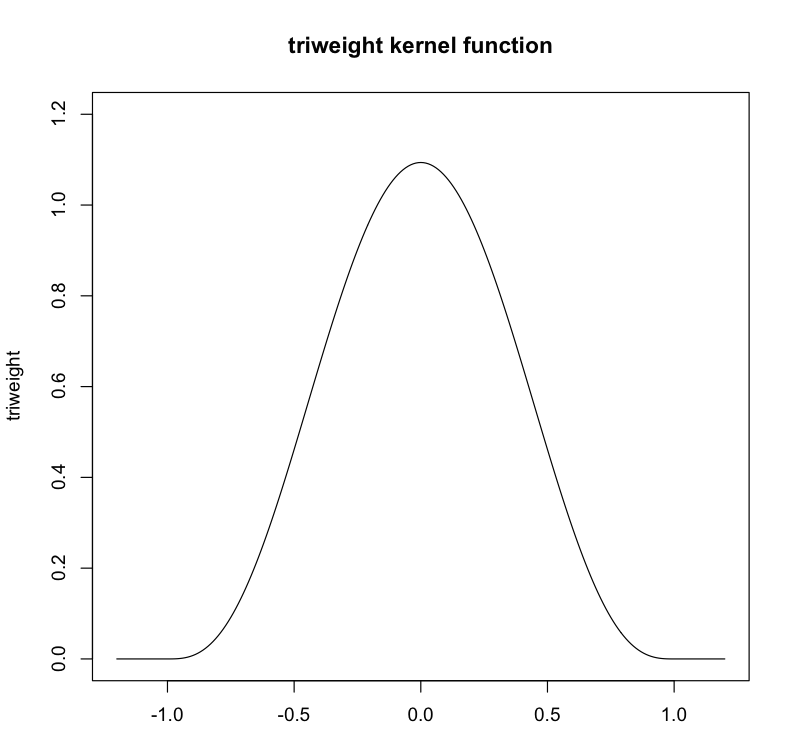
\includegraphics[scale=0.25]{kernelfunction}
    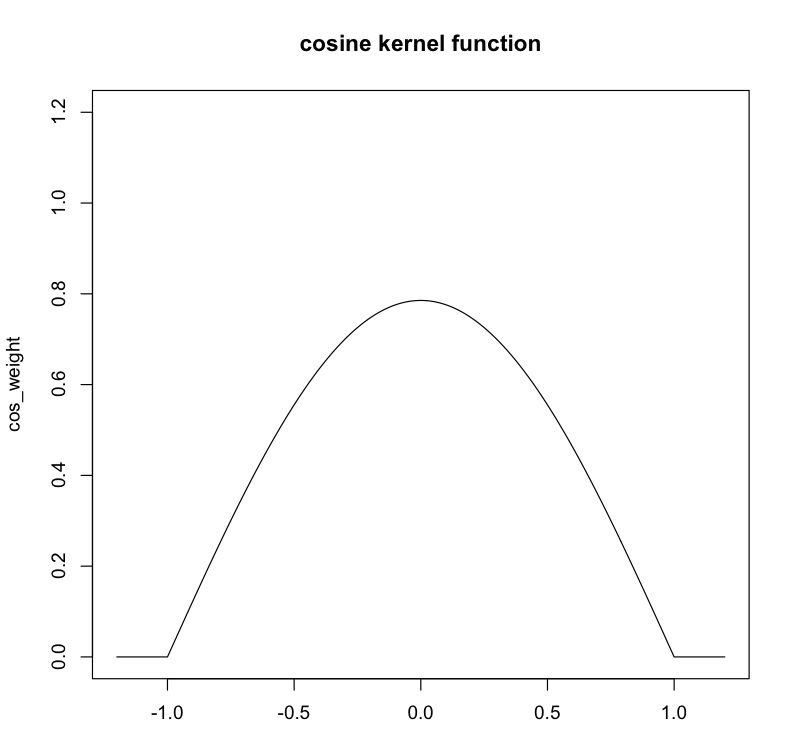
\includegraphics[scale=0.25]{cosinefunction}
    \end{center}

  \item 
    Returning to the wdbc.data data set, use train.kknn to find the 
    optimal kernel function and value of k for predicting breast 
    cancer diagnosis using weighted k-nearest neighbors. 

    The optimal kernel function type for this case is `inv', and the 
    optimal $k$ is 10. 

    \begin{center}
    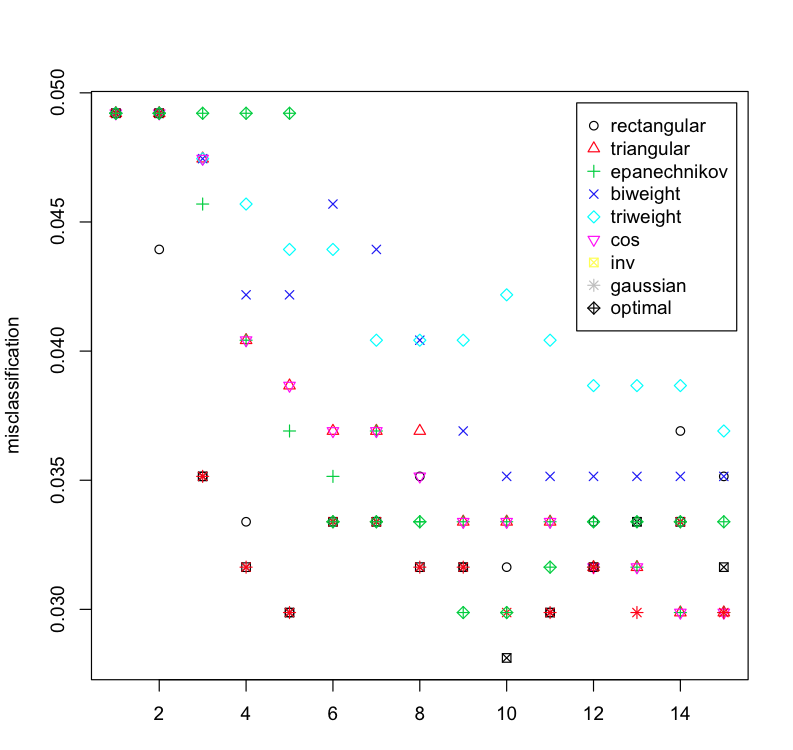
\includegraphics[scale=0.25]{misclass}
    \end{center}
  \item
    Divide the data into 70\% training and 30\% testing data, and 
    calculate the test accuracy using the optimal kernel function 
    and value of k. Find a 95\% confidence interval for the accuracy. 

    The accuracy for this case was 0.977 \%.
    The 95\% confidence interval was (0.9612476 0.9877801).
  \item
    For the same training and test data, find the test accuracy 
    using a rectangular kernel and the optimal value of k obtained 
    in homework 6. 

    The optimal value of k in homework 6 is 4. 
    Using this with the regular knn which gives a rectangular 
    gave an accuracy rate of 0.93 \%.

  \item 
    Test whether the difference in test accuracies is 
    statistically significant. 

    For this run, the p-value is 0.05737. This is borderline, but still 
    greater than 0.05. Thus it is not technically statistically significant 
    although it is close to being so. 

\singlespace
\begin{Verbatim}
#Data Mining hw 7
library(class)
library(kknn)
library(exact2x2)
wdbc <- read.table("~/Dropbox/Tarleton/data_mining/hw05/wdbc.data", 
        header = FALSE, sep = ",")

#1. Use R to plot the triweight and cosine kernel functions from 
#  Hechenbichler and Schliep(2004). Use a plot window of 
#  xlim=c(-1.2,1.2) and ylim=c(0,1.2). 
#  (Hint: Boolean commands like (x <= 20) return TRUE/FALSE values, 
#  but they are treated as 1's and 0's when multiplied by numbers.)

triweight_d = function(x){
  frac = 35/32
  d = frac * ((1 - x*x)^3) * (abs(x) <= 1)
}
x <- seq(from=-1.2,to=1.2,by=0.01)
triweight <-triweight_d(x)
plot(x, triweight, 
     type='l',
     xlim=c(-1.2,1.2),
     ylim=c(0,1.2),
     main="triweight kernel function")

#2. Returning to the wdbc.data data set, use train.kknn to find the 
#   optimal kernel function and value of k for predicting breast 
#   cancer diagnosis using weighted k-nearest neighbors. 

wdbc <-wdbc[,-1]
fit_bc <- train.kknn(V2 ~ ., data = wdbc, kmax = 15, kernel = 
                     c('rectangular', 'triangular', 
                       'epanechnikov', 'biweight', 
                       'triweight', 'cos','inv', 
                       'gaussian', 'optimal'),
                        distance = 2)
plot(fit_bc)
ktype <- (fit_bc$best.parameters)$kernel
k <- (fit_bc$best.parameters)$k

#3. Divide the data into 70% training and 30% testing data, and 
#   calculate the test accuracy using the optimal kernel function 
#   and value of k. Find a 95% confidence interval for the accuracy. 

splitset <- splitdata(wdbc, 0.7, FALSE)
train1 <- splitset$train
pred_V2 = (kknn(V2 ~ ., train = wdbc[train1,], test = wdbc[-train1,], 
           k = k, kernel = ktype, distance = 2))$fitted.values

e1 = (confmatrix(wdbc$V2[-train1], pred_V2))$error
exact_conf_int <- binom.test(nrow(wdbc) - round(e1 * nrow(wdbc), digits = 0), 
                             nrow(wdbc), p = 0.05)

#4. For the same training and test data, find the test accuracy 
#   using a rectangular kernel and the optimal value of k obtained 
#   in homework 6. 

pred_V2_2 = knn(train = wdbc[train1,-1], test = wdbc[-train1,-1], 
                cl = wdbc$V2[train1], 4)

confmatrix(wdbc$V2[-train1], pred_V2_2)

#5. Test whether the difference in test accuracies is 
#   statistically significant. 
acc1 = (wdbc$V2[-train1] == pred_V2)
acc2 = (wdbc$V2[-train1] == pred_V2_2)

mcnemartable = table(acc1, acc2)

mcnemar.exact(mcnemartable)
\end{Verbatim}
\end{enumerate}

\end{document}
